% Figure 19 - MOM object class structure
% Independently revalidated against IEEE Std 1516.1-2010 source physical p.262 / standard p.248.
% Natural source raster: 1792 x 968 pixels. Coordinates below are taken directly
% from that source image; the complete picture is resized as one object by Clause 11.
% Relationship IDs correspond to audit/figure19/relationships.csv.
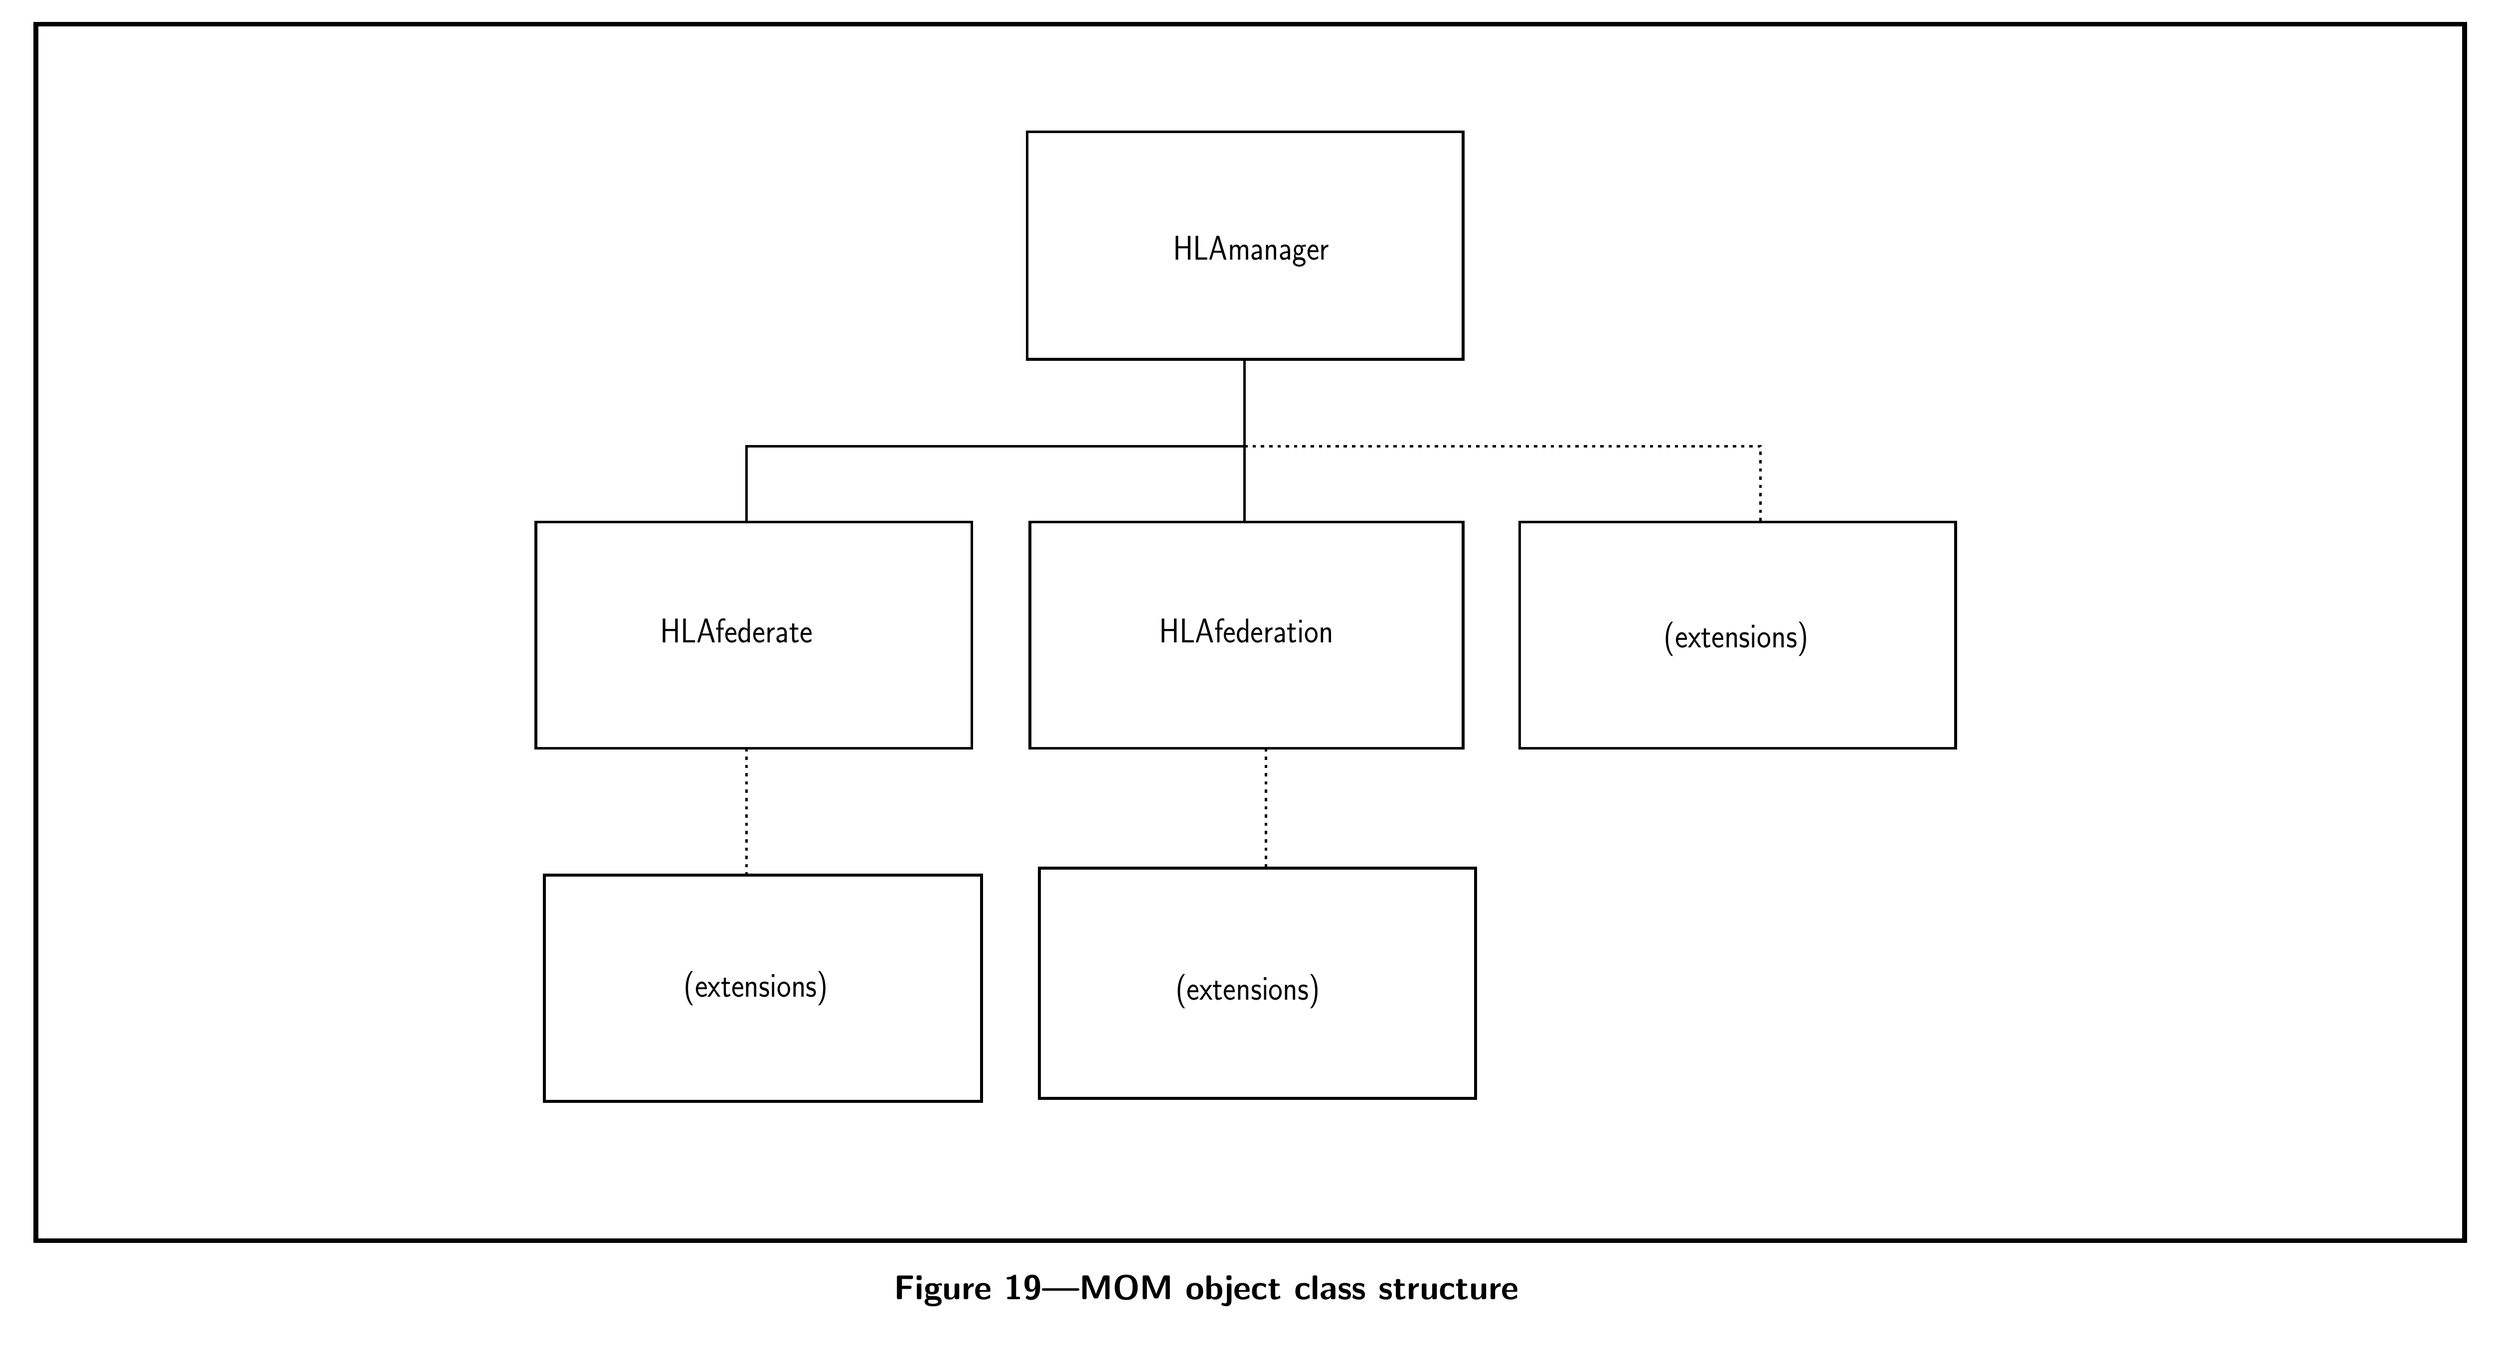
\begin{tikzpicture}[x=1pt,y=-1pt,line cap=butt,line join=miter]
    \path[use as bounding box] (0,0) rectangle (1792,968);

    % Page-local compensation: the reconstruction body text block is slightly left of the source page.
    % A 5-source-pixel shift aligns the native figure frame with source physical page 262.
    \begin{scope}[xshift=5pt]

        % Printed source figure frame.
        \draw[line width=3.4pt] (11,7.5) rectangle (1771.5,889.5);

        % Predefined MOM object-class boxes.
        \draw[line width=2.0pt] (729.5,85.5) rectangle (1045.5,250.5);
        \draw[line width=2.0pt] (373.5,368.5) rectangle (689.5,532.5);
        \draw[line width=2.0pt] (731.5,368.5) rectangle (1045.5,532.5);

        % Extension placeholder boxes.
        \draw[line width=2.0pt] (1086.5,368.5) rectangle (1402.5,532.5);
        \draw[line width=2.0pt] (379.5,624.5) rectangle (696.5,788.5);
        \draw[line width=2.0pt] (738.5,619.5) rectangle (1054.5,786.5);

        % F19-R01: HLAmanager -> HLAfederate, solid predefined hierarchy.
        \draw[line width=1.75pt] (887,250.5) -- (887,313.5) -- (526,313.5) -- (526,368.5);
        % F19-R02: HLAmanager -> HLAfederation, solid predefined hierarchy.
        \draw[line width=1.75pt] (887,313.5) -- (887,368.5);

        % F19-R03: HLAmanager -> direct extension placeholder.
        \draw[line width=1.75pt,dash pattern=on 2.4pt off 3.6pt]
        (887,313.5) -- (1261,313.5) -- (1261,368.5);
        % F19-R04: HLAfederate -> extension placeholder.
        \draw[line width=1.75pt,dash pattern=on 2.4pt off 3.6pt]
        (526,532.5) -- (526,624.5);
        % F19-R05: HLAfederation -> extension placeholder.
        \draw[line width=1.75pt,dash pattern=on 2.4pt off 3.6pt]
        (902.5,532.5) -- (902.5,619.5);

        % Class labels. The exact source raster font is unavailable; Helvetica-family
        % text is horizontally condensed to match the source label widths at page scale.
        \node[font=\sffamily\fontsize{58}{58}\selectfont] at (892.0,172.2)
            {\scalebox{.885}[1]{HLAmanager}};
        \node[font=\sffamily\fontsize{58}{58}\selectfont] at (518.8,447.5)
            {\scalebox{.90}[1]{HLAfederate}};
        \node[font=\sffamily\fontsize{58}{58}\selectfont] at (888.5,447.5)
            {\scalebox{.89}[1]{HLAfederation}};
        \node[font=\sffamily\fontsize{58}{58}\selectfont] at (1243.5,453.5)
            {\scalebox{.891}[1]{(extensions)}};
        \node[font=\sffamily\fontsize{58}{58}\selectfont] at (533.0,706.5)
            {\scalebox{.891}[1]{(extensions)}};
        \node[font=\sffamily\fontsize{58}{58}\selectfont] at (889.5,709.0)
            {\scalebox{.891}[1]{(extensions)}};

        % Native caption, located from the source raster.
        \node[font=\sffamily\bfseries\fontsize{45}{48}\selectfont] at (859.5,926.0)
            {\scalebox{.995}[1]{Figure 19---MOM object class structure}};
    \end{scope}
\end{tikzpicture}
